\chapter{Sobre Reconhecimento de Padrões empregando Aprendizado de Máquina}

\section{Conceitos Gerais}

\section{Extração de Atributos}

\subsection{Local Binary Pattern}



O método usado foi Local Binary Pattern.

Considerações sobre dimensionalidade da imagem.



\section{Classificadores}

Os modelos usados para classificação no sistema foram: Máquina de Vetor de Suporte (SVM, em inglês \textit{Support Vector Machine}) e Floresta Aleatória (\textit{Random Forest Classifier}).

\subsection{Máquina de Vetor de Suporte}

As Máquinas de Vetor de Suporte são um modelo de aprendizado que vem crescendo há um tempo na comunidade de Aprendizado de Máquina e é utilizado em variadas aplicações, desde bioinformática a reconhecimento de imagens, como é o caso desse projeto \citeC{mitchell1997} \citeC{noble2004} \citeC{kim2002}.

Intrinsicamente, o SVM é um modelo de classificação binária em problemas de aprendizado supervisionado (\textit{supervised learning}). Concedido um conjunto de dados para treinamento, todos especificados como pertencendo a uma das duas categorias, o treinamento do algoritmo SVM origina um modelo que irá receber novos dados, julgando-os como de uma categoria ou de outra.

O SVM funciona baseado em um mapeamento de todos os dados de treinamento, representando-os como pontos em um espaço. Os exemplos para treinamento, então, são divididos nesse espaço de acordo com sua categoria de tal forma que os dois conjuntos de pontos estão distanciados por uma lacuna que é a maior possível (Figura \ref{fig:svmDist}). Sendo assim, um novo dado, quando fornecido ao sistema, é mapeado nesse mesmo espaço e é feita a predição de sua categoria de acordo com a sua localização no espaço originado durante o treinamento do modelo.

\begin{figure}[H]
 \centering
  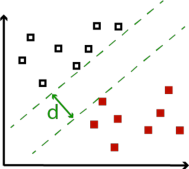
\includegraphics[width=0.4\linewidth]{figuras/svmDist.pdf}
  \caption{Ilustração da distância dos subconjuntos de dados de treinamento mapeados no espaço pelo modelo SVM - \textbf{Fonte:} Autora}
  \label{fig:svmDist}
\end{figure}

Enquanto linear, o SVM pode ser classificado como "Margens Rígidas" ou "Margens Suaves", em ambos casos, definem-se fronteiras lineares no conjunto de dados que aprensentam perfil linearmente separável. Margens são utilizadas no SVM para encontrar a solução de classificação para os subconjuntos de forma que o erro de generalização seja o menor possível. Desta forma, elas são definidas como a menor distância entre o hiperplano (fronteira) de decisão e qualquer uma das amostras de treinamento \citeC{Bishop2006}.

No entanto, apesar de não se aplicar a este projeto, o SVM também pode ser empregado em problemas em que os dados de treinamento não são rotulados, ou seja, em caso de aprendizado não-supervisionado (\textit{unsupervised learning}). Para tal, desenvolveu-se uma nova versão do SVM que também funciona baseada no mapeamento dos dados em um espaço, no entanto, passa-se primeiramente por um processo para encontrar as conexões naturais entre os dados de entrada, formando grupos de acordo com o grau de similaridade apresentado entre eles, para então distribuí-los no espaço. Essa técnica de aprendizado consiste em um algoritmo de aglomeração (\textit{clustering}) e foi nomeada como \textit{Support Vector Clustering} \citeC{ben2001}.

\subsubsection{SVM com Margens Rígidas}

Pode-se definir um conjunto de dados de treinamento como \textit{C}, composto de dados \textit{$x_i$} $\in$ X, onde \textit{i $=$ 1, ..., n} e X é o espaço de dados, cujos rótulos de categoria são \textit{$y_i$} $\in$ Y, onde Y = \{$-$1,$+$1\}. Sendo assim, o conjunto \textit{C} é dito linearmente separável caso possa-se criar um hiperplano tal que os subconjuntos de dados com valor $-$1 seja separado do subconjunto de dados $+$1 \citeC{lorena2007}.

A equação \ref{eq:eqHiper}, representa um hiperplano qualquer e divide o espaço dos dados de treinamento em duas regiões, uma para representar $-$1 e outra, $+$1, sendo $\boldsymbol{w}$ o vetor normal ao hiperplano criado. Desta forma, define-se uma função \textit{$g(x)$} como a função sinal de \textit{$f(x)$} (Equação \ref{eq:eqSgn}) que irá ser o padrão para a classificação de novos dados de entrada.

\begin{equation}
\label{eq:eqHiper}
 f(x)= \boldsymbol{w}\cdot \boldsymbol{x} + b = 0
\end{equation}

\begin{equation}
\label{eq:eqSgn}
 g(x) = sgn(f(x)) =
   \begin{cases}
    +1       & \quad \text{se } w\cdot x + b \text{ } $>$ \text{ } 0\\
    -1  & \quad \text{se } w\cdot x + b \text{ } $<$ \text{ } 0\\
   \end{cases}
\end{equation}

 Para $f(x) = 0$, a distância entre um ponto no espaço (amostra) e o hiperplano definido é dada por $|f(x)| \mathbin{/} ||w||$. Além disso, deve existir pelo menos um conjunto de parâmetros $\boldsymbol{w}$ e \textit{b} que satisfaça \textit{g(x)}, ou seja, tal que \textit{$y_i$$f(x_i)$ $>$ 0}. Sendo assim, pode-se definir a distância entre uma amostra $x_i$ qualquer e o hiperplano escolhido como na equação \ref{eq:eqDist}.

 \begin{equation}
\label{eq:eqDist}
  \frac{y_if(x_i)}{||\boldsymbol{w}||} = \frac{y_i(\boldsymbol{w} \cdot x_i + b)}{||\boldsymbol{w}||}
\end{equation}

As margens ($H_1$ e $H_2$) são definidas, em primeiro momento, mediante a distância perpendicular entre a fronteira de decisão e aquele que é o ponto mais próximo de todas as amostras dos dados de treinamento, como mostra a parte \textit{a} da Figura \ref{fig:marginSVM}. Posteriormente, as margens são maximizadas escolhendo-se a sua localização tomando como base as amostras que se encontram mais próximas do hiperplano separador, como destacado na parte \textit{b} da Figura \ref{fig:marginSVM}. Essas amostras são denominadas Vetores de Suporte (\textit{support vectors}), dando nome à técnica de aprendizado. Para então maximizar a distância entre os vetores de suporte e o hiperplano separador ($f(x) = 0$), deve-se otimizar os parâmetros $\boldsymbol{w}$ e \textit{b}, que serão ajustados durante o treinamento do modelo \citeC{rosebrock2017}.

\begin{figure}[H]
 \centering
  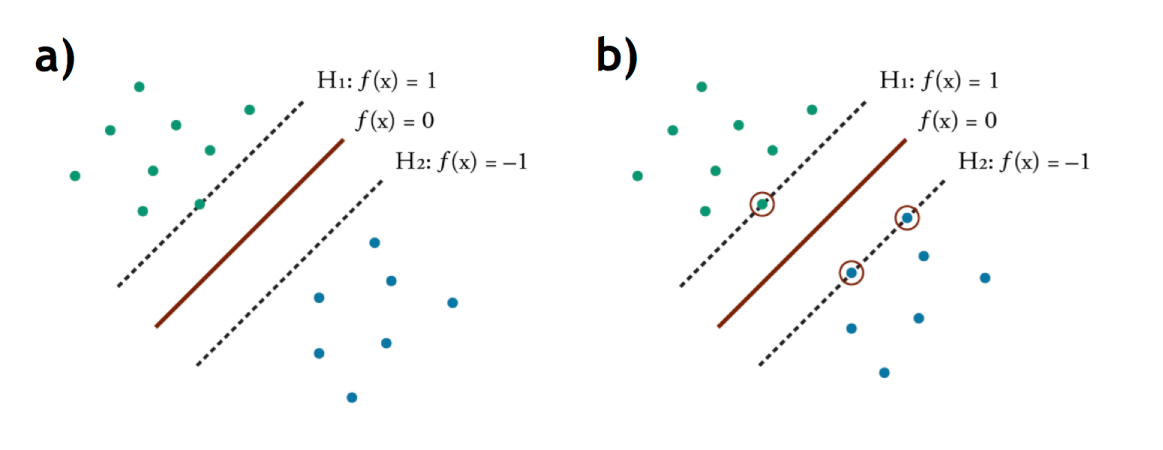
\includegraphics[width=0.9\linewidth]{figuras/marginSVM.pdf}
  \caption{Ilustração do hiperplano separador e do estabelecimento das margens ($H_1$ e $H_2$) no espaço em que os dados de treinamentos estão mapeados - \textbf{Fonte:} Autora}
  \label{fig:marginSVM}
\end{figure}

Dado que realizando um escalonamento, a partir de mesma constante, em $\boldsymbol{w}$ e em \textit{b} não altera-se a distância dos pontos $x_i$ em relação ao hiperplano separador, a expressão $y_i(\boldsymbol{w} \cdot x_i + b)$ pode ser considerada unitária. Desta forma, a distância mínima entre o hiperplano e os dados de treinamento é de $1/||w||$. Busca-se, então, maximizar essa distância com a minimização de $||w||$, valendo-se do problema de otimização na expressão \ref{eq:eqMin}, com as devidas restrições, de forma a garantir que não haverão dados de treinamento entre as margens de separação de classes, daí então a nomenclatura "margens rígidas" \citeC{lorena2007}.

\begin{equation}
\label{eq:eqMin}
  \text{min}\{\frac{1}{2}||\boldsymbol{w}||^2\}
\end{equation}

\begin{equation}
\label{eq:eqRestrição}
  \text{Restrições: } y_i(\boldsymbol{w} \cdot x_i + b) \geq 1, i \in (1,n)
\end{equation}

Isso se torna uma importante propriedade do SVM, tornando a determinação dos parâmetros do modelo uma otimização convexa, na qual a solução mínima é obrigatoriamente a solução global \citeC{Bishop2006}.

Para solucionar o problema de otimização da equação \ref{eq:eqMin}, pode ser utilizada uma função Lagrangiana, associando parâmetros $a_i$ chamados multiplicadores de Lagrange e tornando suas derivadas parciais nulas, a resolução por completo pode ser encontrada em \citeC{Bishop2006} e \citeC{lorena2007}. Valendo-se do resultado dessa operação, tem-se a definição da função utilizada para a classificação dos dados que serão fornecidos ao sistema (Equação \ref{eq:eqSVM}), sendo a função sinal do resultado da função de Lagrange aplicada nesse caso.

\begin{equation}
\label{eq:eqSVM}
  g(x) = sgn(f(x)) = sgn(\displaystyle\sum_{i=1}^{n}a_iy_ik(\boldsymbol{x},\boldsymbol{x_i})+b)
\end{equation}

Pode-se perceber que na Equação \ref{eq:eqSVM} empregou-se o conceito de \textit{kernel} na resolução final do problema de otimização. Define-se a função \textit{kernel} como $k(x,x') = \phi(\boldsymbol{x})^T\phi(\boldsymbol{x'})$, onde por $\phi(\boldsymbol{x})$ denota-se um mapeamento, ou transformação, para um determinado espaço de características (\textit{feature space}), $\phi:X\mapsto\eth$. A função \textit{kernel} recebe dois pontos em um espaço e resulta em o produto escalar de ambos em um novo dado espaço. Apesar de, com o uso da função \textit{kernel} na formulação, o esforço computacional tornar-se mais elevado, dá-se flexibilidade ao modelo, que pode ser reformulado usando diferentes tipos de \textit{kernel} e, então, pode ser aplicado em outros casos nos quais a dimensionalidade excede o número de amostras de treinamento \citeC{Bishop2006}.

\subsubsection{SVM com Margens Suaves}

O SVM com Margens Suaves é uma adaptação da versão com Margens Rígidas para que a aplicação dessa técnica de aprendizado seja mais eficiente em casos reais, os quais, comumente, não se apresentam conjuntos de dados estritamente bem comportados, ou seja, linearmente separáveis. Com essa versão do SVM propõe-se lidar com conjuntos de treinamento mais gerais e, para isso, são concedidas exceções às restrições apresentadas na expressão \ref{eq:eqRestrição}. Sendo assim, são adicionadas ao problema variáveis de folga $\xi_i$, $i \in (1,n)$ e a equação \ref{eq:eqRestrição} é modificada para

\begin{equation}
\label{eq:eqSuave}
 y_i(\boldsymbol{w} \cdot x_i + b) \geq 1 - \xi_i, \text{ } \xi_i > 0, \text{ } i \in (1,n)
\end{equation}

O efeito dessa modificação é que, devido a essa folga adicional, alguns pontos dos dados de treinamento podem permancer entre as margens $H_1$ e $H_2$, porém isso pode gerar erros de classificação \citeC{lorena2007}.

A forma de desenvolvimento do modelo é similar ao SVM com Margens Rígidas, também emprega-se a função de Lagrange, anulando suas derivadas parciais. No entanto, os parâmetros multiplicadores de Lagrange $a_i$ sofrem modificações. A equação \ref{eq:eqMin} é, nesse caso, alterada (Equação \ref{eq:eqMinErro}), e sabe-se que um erro no conjunto de treinamento é indicado por $\xi_i > 1$, portanto, para que o erro gerado por $\xi_i$ seja minimizado, propõe-se a equação \ref{eq:eqMinErro}, onde a constante \textit{K} é um termo de regularização à minimização dos erros no conjunto de treinamento.

\begin{equation}
\label{eq:eqMinErro}
  \text{min}\{\frac{1}{2}||\boldsymbol{w}||^2\ + K\displaystyle\sum_{i=1}^{n}\xi_i\}
\end{equation}

Como no caso anterior, os pontos denominados Vetores de Suporte são aqueles em que a condição $a_i > 0$ é satisfeita. Porém, neste caso, há outros tipos de Vetores de Suporte, denominados livres e limitados, atendem às equações \ref{eq:eqCondicaoMarg1} e \ref{eq:eqCondicaoMarg2} e podem ser vistos na Figura \ref{fig:margemSuave}.

\begin{figure}[H]
 \centering
  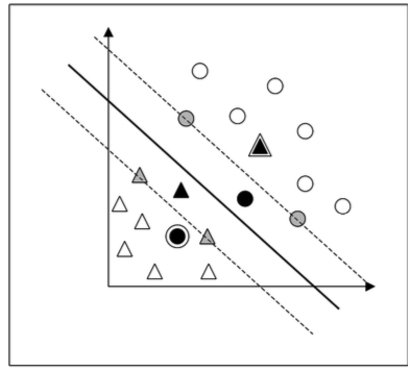
\includegraphics[width=0.4\linewidth]{figuras/margemSuave.pdf}
  \caption{Ilustração dos tipos de vetores de suporte: livres (cinza) e limitados (preto) - \textbf{Fonte:} \citeC{lorena2007}}
  \label{fig:margemSuave}
\end{figure}

Os vetores de suporte chamados livres são aqueles que se encontram exatamente em cima da margem e possuem $a_i \leq K$ e $\xi_i = 0$. Já os vetores de suporte limitados possuem $a_i = K$ e podem ser erros ($\xi_i > 1$) ou pontos classificados corretamente ($0 <\xi_i \leq 1$), porém, que se localizam entre as margens.

\begin{equation}
\label{eq:eqCondicaoMarg1}
 a_i(y_i(\boldsymbol{w} \cdot \boldsymbol{x_i} + b) - 1 + \xi_i) = 0
\end{equation}

\begin{equation}
\label{eq:eqCondicaoMarg2}
 (K - a_i)\xi_i = 0
\end{equation}

Em conclusão, resulta-se na mesma equação de classificação que o modelo anterior (equação \ref{eq:eqSVM}), porém os parâmetros $a_i$ são calculados de forma distinta, com restrições que dependem da constante \textit{K}.

\subsubsection{SVM não-linear}

Apesar de o modelo SVM com Margens Suaves ser mais abrangente do que aquele com Margens Rígidas, ainda trata-se de uma separação de categorias criando um hiperplano, ou seja, depende-se ainda de uma característica linear na distribuição dos dados. No entanto, em aplicações reais, em variados casos o subconjunto de dados não pode ser separado por um hiperplano, como exemplifica a Figura \ref{fig:svmNL}.

\begin{figure}[H]
 \centering
  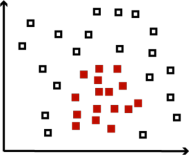
\includegraphics[width=0.35\linewidth]{figuras/svmNL.pdf}
  \caption{Ilustração de conjunto de dados de treinamento que não é linearmente separável - \textbf{Fonte:} Autora}
  \label{fig:svmNL}
\end{figure}

Desta forma, atentando-se para a utilização da função \textit{kernel} na equação \ref{eq:eqSVM}, percebe-se que é possível empregar o SVM em uma classificação não linear, empregando um "truque de \textit{kernel}" { }(\textit{kernel trick}) que se resume em mapear os dados de entrada em um espaço com dimensão superior, denominado espaço de atributos (\textit{feature space}), apresentado na Figura \ref{fig:svmKernel} \citeC{shawe2004} \citeC{boser1992}. Logo, tem-se $\phi:X\mapsto\eth$, onde $\eth$ é o novo espaço de características e nota-se que o bom desempenho do classificador depende de uma escolha apropriada de $\phi$, de modo que realmente possa ser realizada uma divisão linear nos dados de treinamento.

\begin{figure}[H]
 \centering
  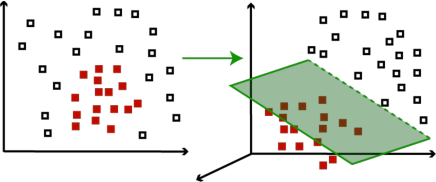
\includegraphics[width=0.75\linewidth]{figuras/svmKernel.pdf}
  \caption{Ilustração de mapeamento de conjunto de dados de treinamento em novo espaço de características a partir da utilização de função \textit{kernel}, possibilitando a divisão linear entre as categorias - \textbf{Fonte:} Autora}
  \label{fig:svmKernel}
\end{figure}

Para haver alta probabilidade de que os dados mapeados para o novo espaço de características seja linearmente separável, duas condições devem ser satisfeitas, segundo o teorema de Cover \citeC{cover1965}. Primeiramente, a transformação ($\phi$) deve ser não-linear e, em segundo lugar, a dimensão do espaço de características deve ser suficientemente alta.

No processo de treinamento, ocorre o mapeamento dos dados de treinamento para o espaço de característicias aplicando-se $\phi$ no conjunto de dados e, por obter um melhor desempenho em relação a ruídos, emprega-se o SVM com Margens Suaves. Após isso, as equações para otimização são calculadas, porém com a aplicação do operador $\phi$. Sendo assim, o classificador é descrito na equação \ref{eq:eqSVM}.

Comumente, aplica-se o \textit{kernel} sem necessarimente a ciência do operador $\phi$, deixando-o como uma operação implícita durante o treinamento. Esse é mais um motivo para usar-se a função \textit{kernel}, por se tratar de um operador que provê um cálculo simples (produto escalar) e representa bem espaços. Para garantir que as condições expostas anterioremente nessa seção sejam cumpridas, utilzam-se alguns tipos de \textit{kernel} que satisfazem as condições de Mercer. Todos aqueles que foram utilizados neste projeto são apresentados na Tabela \ref{tab:svmkernel}.

\begin{table}[h]
 \centering
 \begin{tabular}{l|c|c}
    Tipo & Função $k(x,x')$ & Parâmetros\\
  \hline
  Linear &  $(\delta(x \cdot x') + \kappa)$ & $\delta,\kappa$ \\
  Polinomial &  $(\delta(x \cdot x') + \kappa)^d$ & $\delta,\kappa, d$  \\
  RBF & $\exp(\frac{-||x - x'||^2}{2\sigma^2})$ & $\sigma$ \\
  Sigmoidal & $\tanh(\delta(x \cdot x') + \kappa)$ & $\delta,\kappa$ \\
 \end{tabular}
 \caption{Resultados de acurácia em testes de validação cruzada do sistema com o modelo SVM avaliado com diferentes \textit{kernels} em banco de imagens completo - \textbf{Fonte:} \citeC{lorena2007} e \citeC{martin2012}}
 \label{tab:svmkernel}
\end{table}

\subsubsection{SVM Multiclasse}

Apesar de se tratar de um classficador que é intrinsicamente binário, o SVM pode também ser aplicado em problemas que apresentem várias categorias. Para tal, foram desenvolvidas ao longos dos anos novas soluções para a multiclassificação a partir de combinações múltiplas do classificador binário explicitado previamente nessa seção. Alguns modelos de adaptação do SVM para variadas classes são Um-contra-um (OvO, em inglês \textit{one vs. one}), Gráfico Acíclico Dirigido (DAG, em inglês \textit{Directed Acyclic Graph}), Código de Correção de Erro de Saída (ECOC, em inglês \textit{Error Corrected Output Coding}) e Um-contra-todos (OvA, em inglês \textit{One vs. All}), sendo este utilizado neste projeto.

Supondo que um conjunto de dados possui $m$ classes para ser classificado, empregando a abordagem Um-contra-todos, um total de $m$ classificadores binários SVM devem ser criados para efetuar a classificação de uma determinada categoria em relação às demais $m-1$. Então, no momento de testes ou de classificação de novos dados, esses são classificados criando-se uma margem a partir do hiperplano separador e a classe daquela nova amostra corresponde ao SVM que possui a maior margem dentre os demais \citeC{pal2008} \citeC{Bishop2006}.

Sendo assim, para um problema deste tipo, devem ser determinados $m$ hiperplanos, consequentemente, requere-se solução de $m$ problemas de otimização, sendo que, em cada um deles uma classe, é separada das demais. Desta forma, configura-se uma desvantagem dessa abordagem, já que, durante a fase de treinamento, há um processo computacionalmente oneroso. Ademais, supondo que todas as classes possuam uma quantidade igual de amostras para treinamento, durante esse processo, já que o SVM se comporta como um classificador binário, uma classe terá bem menos amostras para treino do que a outra classe, apresentando a razão $1:(m-1)$ \citeC{pal2008}.



\subsection{Floresta Aleatória}








